\documentclass{sig-alternate}
\usepackage{algorithmic}
\usepackage{pseudocode}
\usepackage{fancybox}

\newtheorem{hyp}{Hypothesis}

\title{CS 472 --- Project 3}
\subtitle {GAs \& DEs --- A Land of Lisp Approach}

\numberofauthors{1}

\author{
\alignauthor
Steven White \\
  \email{swhite24@mix.wvu.edu}\\
  8258
}

\begin{document}
\date{22 March 2012}
\pagenumbering{arabic}

\maketitle
\section{abstract}

\subsection{Introduction}
Introduces problem description and intent of study.

\subsection{Models}
Describes Conrad Barski's \emph{Land of Lisp} model in detail.  Outlines modifications made to model to suit purposes of this study.

\subsection{Algorithms}
Compares and constrasts differential evolution with genetic evolution with pseudo-code.

\subsection{Expectation}
Lays out four hypothesis indicating what is expected of study.

\subsection{Results}
Displays results in tables and figures and also elaborates on the data.

\subsection{Validity}
Comments on the degree which the results are valid.

\subsection{Conclusion}
Evaluates each hypothesis based on results.

\subsection{Further Work}
Lays out further steps to take to improve study.

\section{Introduction}
\label{sec:Introduction}
The purpose of this project is to objectively compare two subsets of evolutionary algorithms, differential evolution (DE) and genetic algorithms (GA), using the model of evolving rats found in Conrad Barski's \emph{Land of Lisp}.  The two sets of algorithms will be tested for success in several criteria --- run-time, diversity of population, scoring, and time taken to achieve a stable population.

The algorithms will be tested with both a single-objective and multiple-objective version of the evolving rats problem.  The simplest and most obvious objectives to use in the context of this problem are the amount of energy a candidate has in comparison to the maximum potential energy and the number of children a candidate has produced relative to its age.  Due to the nature of these objectives and the model itself, a slight diversion was made from the traditional versions of DEs and GAs which immediately compare the scores of candidates with parents.  Instead, we will allow the candidates free roam for a period of generations, in order to be able to accurately assess their success.  Once a candidate is of correct of age, it will be compared with its parent.  Each objective will be scored independently and will be unweighted.  If a candidate dominates the parent, the parent will be removed from future generations.  Conversely, if a candidate is dominated by the parent, the candidate will be removed.  If neither the parent nor the candidate dominate the other, both will remain for future generations.

In addition to comparing one algorithm set with the other, each set will be compared to itself by changing their corresponding choice options, such as scaling factor when mutating and the number of objectives to be scored.  Changing these options will affect each of the previously listed comparative criteria and may also arrive at a better solution.

\section{Model}
\label{sec:Model}
\subsection{World Description}
The model to be used for both differential evolution and genetic algorithms will be the rat evolution model of \emph{Land of Lisp}.  This model evolves a randomly generated initial population of a single rat.  The landscape of the ``world'' is thirty units tall by one hundred units wide.  The rats are herbivores, and the landscape is populated with two additional plants for each generation.  Rats have a set amount of energy, and must find plants to regain lost energy in order to remain alive.  Should a rat's energy reach zero, the rat will die and be removed from further generations.  A central ``oasis'' is present in the landscape.  Of the two plants placed in the landscape for each generation, one will be placed randomly inside the oasis, and the other placed randomly somewhere outside the oasis.  Figure 1 depicts a visual representation of the landscape with a central oasis. \cite{LOL}
\begin{figure}
\centering
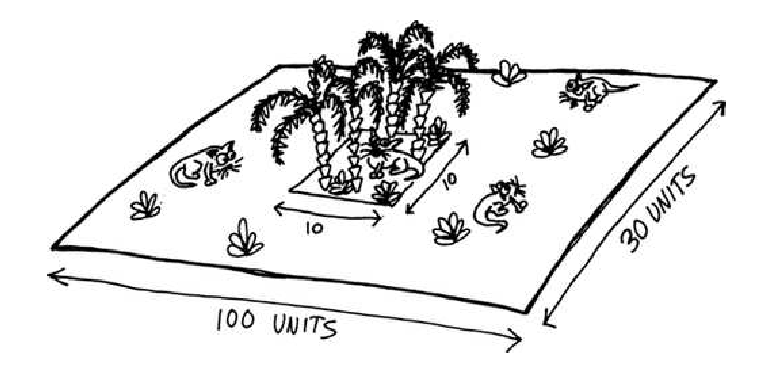
\includegraphics[width=0.4\textwidth]{landscape.PNG}
\caption{Visual representation of rat ``world''.}
\end{figure}

Each generation of this model involves a specific life-cycle of the rats.  The first thing rats do is turn.  The direction of the turn is determined by the rat's genes.  Each rat has a set of genes corresponding to how likely they are to turn a certain direction.  A visual depiction of this these genes and their corresponding directions is shown in Figure 2.  \cite{LOL}
\begin{figure}
\centering
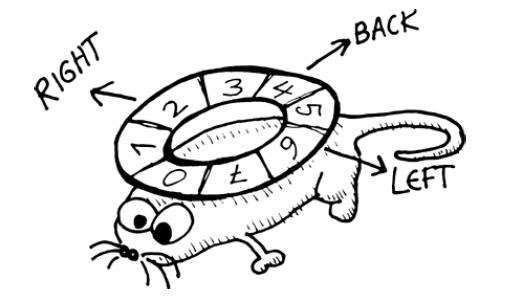
\includegraphics[width=0.4\textwidth]{rat_wheel.PNG}
\caption{Gene ``wheel'' depicting directions of rat travel.}
\end{figure}
For example, a rat with higher values in the lower-indexed positions of the gene will make less dramatic turns.  

Once turned, the next step in a rat's life-cycle is to move in the specified direction.  Due to the centrally located oasis, two distinct types of genes are expected to evolve.  The first will have higher valued genes with lower indexes, causing them to run at a more constant direction and often returning to the oasis.  The second will have higher valued genes with higher indexes, causing them to wander around a fairly consistent area, i.e. the oasis.  

The final step in the life-cycle of a rat is to produce offspring.  Offspring is produced froma single parent, similar to DE.  This implies that GAs will have no cross-over, only mutation.  In order for a rat to be eligible to reproduce, a minimum energy requirement must be met.  Should that requirement be met, the total energy of the parent is split equally between itself and the offspring.  The genes of the offpring are uniquely generated by each algorithm, though a basic premise remains that offpsring are similar, but typically not identical, to their parent.

\subsection{Modifications for our Purposes}
Unlike the original version, the model used for all experiments described later had an initial population of four rats.  The primary reason for this difference is that differential evolution requires the parent and three other randomly generated rats for the parent to produce offspring.  An initial population of just a single rat would prevent any diversity in the population of rats, merely a horde of clones.  The same setup was used for genetic algorithms simply for consistency.

Staying true to traditional evolutionary algorithms, offspring will compete with parents for a position in the population for future generations.  Once a child is of sufficient age, it will be scored and compared to its parent, with the individual with a better score living on.  This presents two distinct possibilities of rats being terminated, natural dying by running out of energy as well as being ``killed off'' by either a parent or child.  This is different from the original model in which rats only died if their energy reached zero.  

\subsection{Decision Space}
The decision space of this model consists entirely of the genes of each rat.  No other controllable factor has so large an effect on the success of an individual.  The genes are what determine direction of travel, and ultimately what areas of the landscape are covered by each rat.  This facilitates the natural killing off of animals with bad genes, since they will travel in patterns not ideal for this model, as well as allowing the rats with better genes to flourish, since they will frequently encounter plants in the landscape to devour.

The method in which genes are tweaked is unique to each algorithm.  Differential evolution uses a single parent and three additional randomly generated members of the population to create a candidate using cross-over and mutation.  Our genetic algorithm uses only mutation and not crossover, despite traditional GAs performing crossover, due to crossover requiring two parents and this model reproduces asexually.

\subsection{Objective Space}
Two objectives were decided upon for these experiments.  The first is an energy-score.  This may initially seem like a peculiar choice since parents and their offspring start with the same amount of energy.  However, since children are given a specific period of time to live before being compared to their parent, often the child or the parent will be able to further consume plants or reproduce, resulting in different amounts of energy.  The energy-score for each rat is to maximized, up to a value of 1.  The calculation of the energy objective is as follows.

\begin{displaymath}
energyScore = currentEnergy / maxEnergy
\end{displaymath}

The second objective for these experiments involves the number of times a rat is able to produce offspring.  This objective may seem to favor the parents, due to them being alive longer, however the score is not determined solely on the number of offspring.  In order to put offspring on a level ground with parents, the number of offspring is divided by the age in terms of generations alive.  This result yields a maximum value of one, the best score, and is calculated as follows.

\begin{displaymath}
reproductionScore = numberOfChildren / ageOfRat
\end{displaymath}

Since each of these two objectives are to be maximized, an ideal rat will always have the maximum amount of energy and reproduce in every generation.  This, however, is impossible due to the nature of this model.  While maximizing each objective would contribute to the overall success of an individual rat, the objectives compete with one another.  Hoarding energy means the rat is not reproducing regularly and, conversely, reproducing at a high rate will result in a lower amount of energy.  

\section{Algorithms}
\label{sec:Algorithms}

\subsection{Genetic Algorithm and Differential Evolution Similarities}
When comparing GAs with DEs there are multiple apparent similarities.  Firstly, each algorithm requires a randomly generated initial population.  The size of this initial population sets a limit on the maximum population size for all subsequent generations.  Each member of the population will produce a candidate, which is where the primary difference between the two lies.  Ordinarily, this candidate is then compared with its ``parent'' based on some pre-defined objective criteria, and the winner is then reinserted back into the population with the loser begin discarded.  However, as described previously, for our purposes the child rat will be given a set period of time to live before being compared with its parent.  A modified version of the basic outline for DE can adequately describe the similarities of each algorithm and is shown below.\cite{DEMO}

\begin{pseudocode}{DEandGA}{ }
\mathcal{P} \GETS \mbox{randomly generated initial population}\\
\WHILE \mbox{stopping criterion not met} \DO
\BEGIN
\FOREACH member \in \mathcal{P} \DO
\BEGIN
\IF \mbox{member is old enough}
\THEN \mbox{compare to parent and keep better}\\
\mbox{generate candidate from member, add to } \mathcal{P}
\END
\END
\end{pseudocode}

Another commonly used algorithm for each algorithm is the method which shows a summary of the living population of rats.  This is used to look for distinct populations of rats in the population.  Algorithm 4.2 describes the procedure and is shown below.

\begin{pseudocode}{PopulationSummary}{ }
x \GETS \mbox{array of 8} \\
\FOR i \GETS 1 \TO length(all\_rats) \DO
x \GETS x + all\_rats[i]\\
\ENDFOR
\FOR i \GETS 1 \TO 8 \DO
x[i] \GETS x[i] / length(all\_rats)\\
\ENDFOR
\RETURN{x}
\label{alg:populationsummary}
\end{pseudocode}

The generation of candidate from each member of the population is what distinguishes the two algorithms from each other.  The following two sections describe how each algorithm produces a candidate.

\subsection{Genetic Algorithms}
All genetic algorithms use two operators to generate new candidates for the population, crossover and mutation.\cite{Konak:GA}  Crossover involves combining two ``parents'' to produce an offspring.  There are several different varieties of crossover, such as single-point crossover and multi-point crossover.  Mutation randomly changes the offspring produced from crossover, typically by a small amount.  The main purpose of mutation is to introduce a larger amount of diversity in the population.  The GA procedure used to generate offspring in our experiments is shown below.\cite{Konak:GA}

\begin{pseudocode}{GA\_Candidate}{\mbox{Parent p}}
n \GETS \mbox{random integer from 1 to 8}\\
candidate \GETS p\\
candidate \GETS candidate \mbox{ (with gene } n \mbox{ modified by f)}\\
\RETURN{candidate}
\end{pseudocode}

Once an offspring rat is created, it is allowed to live freely for a set period of time before being scored and compared with its parent.  Once this free period expires, the offspring is compared with its parent and if it scores better, it remains in the population and replaces the parent.  If it does not score better, it is discarded.

\subsection{Differential Evolution}
Differential evolution uses crossover, similar to genetic algorithms.  However, DEs do not use mutation, and instead generate an offspring from three random individuals from the population other than the parent.  The randomly generated offspring then undergoes crossover with parent using a predefined crossover probability.  The outline of generating a candidate with DE is shown below.\cite{DEMO}

\begin{pseudocode}{DE\_Candidate}{\mbox{Parent p}}
\PROCEDURE{Candidate1}{x,y,z}
candidate \GETS x + f*(y-z)\\
\RETURN{candidate}
\ENDPROCEDURE
\MAIN
x,y,z \GETS \mbox{random members of }\mathcal{P}\\
candidate \GETS \CALL{Candidate1}{x,y,z}\\
\mbox{Modify $candidate$ by binary crossover with $p$}\\
\RETURN{candidate}
\ENDMAIN
\end{pseudocode}

Once a candidate offspring is produced it is given a period of free life, similarly to how GAs are treated, instead of being immediately compared with the parent.  If the candidate is better than the parent, the parent is replaced, otherwise the candidate is discarded.

\section{Expectations}
\label{sec:Expectations}
\begin{hyp}
\begin{minipage}[t]{2.2 in}
Due to the location of newly created plants in the rat landscape, the rats who frequently visit the center ``oasis'' will have a higher chance of survival.  This will lead to two groups of rats: those who roam around the oasis, and those who run loops around the landscape.
\label{hyp:groups}
\end{minipage}
\end{hyp}

Hypothesis 1 predicts that two distinct groups of rats should arise after a sufficient number of generations.  This prediction was originally presented by Conrad Barski in the description of the rat model.\cite{LOL}  His reasoning for the model forming two groups of rats is that the most successful rats will frequently visit the central oasis of landscape, which gets significantly more plants to consume than any other portion of the landscape.  The first anticipated group will have higher values in the latter portion of their genes, resulting in them frequently doing an about face and remaining in the landscape for the majority of their lives.  The second group will have higher values in the earlier portion of their genes, resulting in very little turning doing complete revolutions around the landscape and traveling through the oasis on each revolution.

\begin{hyp}
\begin{minipage}[t]{2.2 in}
Genetic Algorithms will execute faster than Differential Evolution for all combinations of the number of generations and the number of objectives.
\label{hyp:faster}
\end{minipage}
\end{hyp}

Hypothesis 2 predicts that genetic algorithms will execute faster than differential evolution no matter the number of objectives use to score the rats or the number of generations conducted.  This prediction is based on the fact that differential evolution requires a total of four members of the population in order to produce a new candidate\cite{Das:DE}, whereas genetic algorithms require only a single parent.  The additional members of the population require more processing time to obtain.

\begin{hyp}
\begin{minipage}[t]{2.2 in}
Differential Evolution will approach the two population hypothesis in fewer generations than Genetic Algorithms.
\label{hyp:defaster}
\end{minipage}
\end{hyp}

Hypothesis 3 predicts that differential evolution will arrive at the two dominant populations of rats described in Hypothesis 1 in fewer generations than genetic algorithms.  The method in which differential evolution produces new candidates, by using three members of the population to produce an initial candidate and then a binary crossover with a parent, allows for more diversity in the population.  The specific genetic algorithm used in this experiment uses only a single parent's genes with mutation, resulting in less diversity.

\begin{hyp}
\begin{minipage}[t]{2.2 in}
Both algorithms will maintain a similar number of living rats after a sufficient amount of generations due to the natural killing off rats in the model.
\label{hyp:livingrats}
\end{minipage}
\end{hyp}

Hypothesis 4 predicts that each algorithm will result in a fairly constant number of living rats after a sufficient number of generations.  The natural starving off of rats in this model, occuring when a rat reaches an energy level of 0 by not consuming enough plants, puts an implicit population cap on the rats.  The cap is also affected by the size of the landscape, a mere 100 units by 30 units, as well as the number of new plants introduced to the landscape, two new plants for each generation.\cite{LOL}  The small size and number of plants is not compatible with a large population, and as such the number of living rats will be limited.

\section{Results}
\label{sec:results}
Performance, effectiveness, better on one or multiple
objectives.  Graphs, etc.

\subsection{Test Problem}
The problem tested in our experiments is that of evolving rats from Conrad Barski's \emph{Land of Lisp} described in detail in section~\ref{sec:Model} on page~\pageref{sec:Model}.  The constraints on world size, oasis size, and number of plants introduced to the landscape per generation are followed exactly.  Each algorithm, when compared with the other, also uses the same value of scaling factor and mutation rate.

\subsection{Performance Measures}
\label{sec:perf}
The performance measures used in our experiments are quite simple in nature.  The first is the \emph{Average gene metric}.  This metric calculates the average gene of all living rats in the landscape, then determines the percentage of total genes found in each specific gene.  These percentages allow an observer to look for patterns in the types of rats still living.  For example, an \emph{Average gene metric} with larger percentages in lower-indexed portion of the gene would indicate a rat population with the majority favoring a behavior involving little to no change of direction, resulting in frequent revolutions of the landscape.\cite{LOL}  

The second performance metric used is the \emph{Number of living rats}.  This metric determines if the algorithm has any affect on the number of living rats outside of the already existing constraints put in place by the problem itself, such as the limited size of the landscape and limited amount of plants.  

The third performance metric used is the \emph{Time of execution}.  This metric simply measures the run-time of each algorithm for different numbers of generations.

\subsection{Results of Experiments}
Table~\ref{tab:livingrats} on page~\pageref{tab:livingrats} illustrates the number of living rats for each algorithm for different numbers of conducted generations. It adequately demonstrates how each the initial population of rats, 10,000, quickly decreases to the natural population limit put in place by the model.  It shows that neither algorithm, using single or multiple objectives, puts any additional constraint on the population.

\begin{table*}
\centering
\caption{Average number of living rats by generation}
\label{tab:livingrats}
\begin{tabular}{c|c|c}
Number of Generations & Number of Living Rats-DE & Number of Living Rats-GA \\
\hline
0 & 10,000 & 10000\\
100 & 40,013 & 40,012\\
200 & 210 & 215\\
300 & 95 & 85\\
400 & 70 & 71\\
500 & 84 & 79\\
600 & 79 & 78\\
700 & 85 & 81\\
800 & 91 & 95\\
900 & 86 & 91\\
1,000 & 83 & 84
\end{tabular}
\end{table*}

Figure~\ref{fig:avggene} on page~\pageref{fig:avggene} shows the average gene, in percentages of the total gene, for each algorithm using both single and multiple objectives.  This metric shows all four variants having two ``humps'' in the genes of the population, with genetic algorithms and differential evolution having stark differences in degrees.  The two ``humps'' associated with genetic algorithms contain a much larger portion of the genes in the humps, indicating two very different types of rats in the population, whereas the two ``humps'' associated with differential evolution make up only a mild increase of the total genes, indicating a more uniform population.

\begin{figure}
\centering
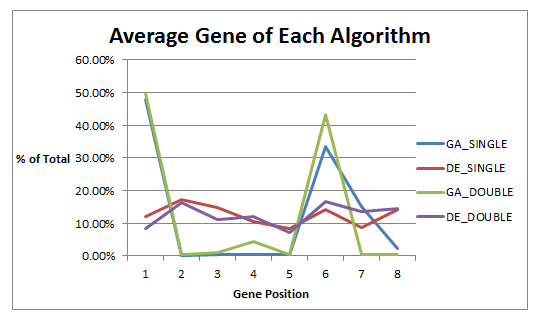
\includegraphics[width=0.5\textwidth]{avg_gene.png}
\caption{Average gene for each algorithm, indicating two populations.}
\label{fig:avggene}
\end{figure}

Figure~\ref{fig:runtimes} on page~\pageref{fig:runtimes} shows four graphs depicting the runtimes of single-objective GA, multi-objective GA, single-objective DE, and multi-objective DE.  The first two graphs show GA against DE on both a single objective and multiple objectives, and they depict a clear difference in the runtimes, with genetic algorithms performing significantly better than differential evolution for both versions.  This is to be expected as differential evolution has more processing involved with the creation of new candidates.  The second two graphs compare the runtime difference of single objective and multiple objectives for each algorithm.  These graphs show a consistent increase in the runtime of multiple objectives, though perhaps not to the degree one would expect.

\begin{figure*}
\centering
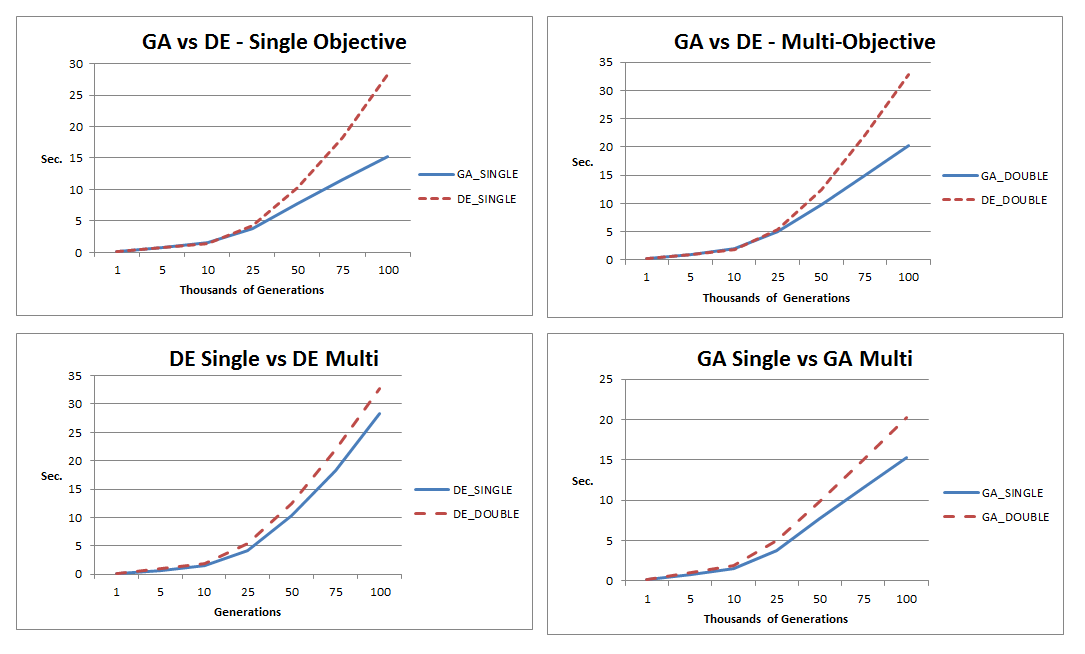
\includegraphics[width=1.0\textwidth]{runtimes.png}
\caption{Comparison of runtimes for each algorithm and objective type.}
\label{fig:runtimes}
\end{figure*}

The final set of results obtained in this study is the number of generations required for each algorithm to portray a consistent grouping pattern in the average genes of the rat population.  These results show that genetic algorithms took on average 20,000 generations whereas differential evolution took on average 15,000 generations to produce a pattern.  

\section{Validity}
Comment on limitations of study.
\subsection{Conclusion Validity}
The degree to which conclusions made about relationships between variables in this experiment are justified is mostly sound.  Concluding that genetic algorithms execute faster than differential evolution can be done simply by observing the statistic directly involved, time of execution.  The same can be said for concluding that neither algorithm will have enough of an affect on the population size to overcome the already in place constraints by the problem itself.  This can be determined simply by observing the number of living rats.

The third conclusion made on the two groups of rats forming in the population, however, is not as direct.  The basis for this conclusion is the \emph{Average gene metric} described in section~\ref{sec:perf} on page~\pageref{sec:perf} and calculated via algorithm \ref{alg:populationsummary} on page \pageref{alg:populationsummary}.  This procedure returns a list of the percentages each individual gene makes up of the total.  These percentages are then used to infer the movement tendencies of the living rats in the populations and group them into ``sub-species''.  The use of this metric comes from Conrad Barski's \emph{Land of Lisp} where he describes how the genes of the rats indicate distinct patterns.\cite{LOL}

\subsection{Internal Validity}
The internal validity of this study is quite good.  The different experiments use the same variables for each algorithm and then make conclusions based on the results.  Each algorithm is also compared to itself while changing only one parameter and keeping all others constant, allowing for a higher degree of internal validity.

\subsection{Intentional Validity}
The chosen model, described in section~\ref{sec:Model} on page~\pageref{sec:Model}, is sufficient in assessing the effectiveness of both differential evolution and genetic algorithms, due to it having multiple potential objectives to be optimized.  The only drawback of this model is the natural decreasing of population size.

Since the purpose of this study is to compare genetic algorithms with differential evolution in terms of runtimes and effectiveness arriving at an optimal solution, the metrics described in section~\ref{sec:perf} on page~\pageref{sec:perf} adequately assess each of those goals.
 
\subsection{External Validity}
The degree of external validity of this study is quite high since the model used behaves the same for each algorithm.  Performing this same study on a different model would yield similar results.

\subsection{Ecological Validity}
The nature of this study, comparing and constrasting genetic algorithms with differential evolution, allows for a high degree of ecological validity since there are no ethical concerns involved with the assessment of algorithms.  The rat evolution model used in this study, however, may present some concerns if offspring are expected to compete with parents for a spot in future generations.

\section{Conclusion}

Based on the results described in section~\ref{sec:results} on page~\pageref{sec:results}, Hypothesis~\ref{hyp:groups} can be confirmed.  This hypothesis predicted that two groups of rats would arise as the dominant groups: those who roam around the central oasis, and those who run circles around the landscape and frequently visit the oasis.  Figure~\ref{fig:avggene} shows that two ``humps'' are present in the average genes of the rat population for both single and multiple objective versions of each algorithm, indicating the presence of two majority groups.  The hump with in earlier portion of genes represents the rats who rarely turn from their present direction of travel, and consequently run circles around the landscape.  The hump in the latter portion of genes represents the rats who frequently turn back on their current direction of travel, resulting in them staying in a very specific section of the landscape, the oasis.

Hypothesis~\ref{hyp:faster}, predicting that GAs will execute faster than DEs, can also be confirmed based on the results displayed in Figure~\ref{fig:runtimes}.  This figure shows a graphical representation of the runtimes for single and multiple objective versions of both genetic algorithms and differential evolution, with GAs performing better in both after a sufficient number of generations.  GAs and DEs appear to perform similarly for smaller numbers of conducted generations, but as the number of generations grows the difference in performance begins to swing more and more into the favor of GAs.  A second inference can also be made based on this figure --- that the difference between GAs and DEs is greater than that of single objective and multiple objective.

Hypothesis~\ref{hyp:defaster} can be partially confirmed based on the results.  This hypothesis predicted that differential evolution will arrive at two distinct populations in fewer generations than genetic algorithms.  The two population grouping of the rats is in fact observable at an earlier generation in differential evolution, around generation 15,000, than that of genetic algorithms, around generation 20,000.  However, the difference is not nearly as great.  As shown in Figure~\ref{fig:avggene} on page~\pageref{fig:avggene}, the degree to which the genes representing the two populations stand out from the remainder of the genes is much greater in GAs than in DEs.  This implies that GAs result in populations that are much more diverse.

Finally, Hypothesis~\ref{hyp:livingrats}, predicting that both genetic algorithms and differential evolution will have similar numbers of living rats after a sufficient number of generations, can be confirmed as well.  Table~\ref{tab:livingrats} on page~\pageref{tab:livingrats} shows the number of living rats present when conducting either genetic algorithms or differential evolution for generations ranging from 0 to 1,000.  The initial population of rats is constant for both algorithms, and after approximately generation 200 the number of living rats sharply declines.  This decline is a result of rats having their energy values decreased to 0, a constraint put in place by the model itself, and does not relate to either algorithm.

\section{Further Work}
One beneficial next step to take following this study is to observe how changing some of the specifics of the model used affects the final population of living rats.  One of these variables to change would be the size of the landscape and/or oasis.  Changing this would affect the density of plants in the landscape, and perhaps alter the types of rats that would be successful.  A second variable to change would be the rate which new plants are introduced to the landscape.  Changing this variable would also affect plant density.

A second step to take would be to alter the internal variables that affect offspring generation for each algorithm, such as mutation rate, scaling factor, and/or crossover frequency.  Altering these values would affect the type of offspring produced and ultimately the population as a whole, although the effect will likely be profound in DE due to it using both scaling factor and crossover frequency.



\bibliographystyle{plain}
\bibliography{report}

\section{Listings}
All source code and example output is provided below.


\end{document}
